\documentclass[a4paper,12pt]{report}
\usepackage{graphicx}
\usepackage{tikz}
\usepackage{float}
\usepackage[document]{ragged2e}
\usepackage[utf8]{inputenc}
\usepackage[T1]{fontenc}
\usepackage[spanish]{babel}
\renewcommand{\shorthandsspanish}{}
\usepackage{xurl}

\usepackage{listings}

\begin{document}

\begin{titlepage}
	\begin{tikzpicture}[overlay, remember picture]
		\path (current page.north east) ++(-0.3,-1.5) node[below left] {
\includegraphics[width=0.4\textwidth]{/home/saikkopat/Documents/LOGOS IPN/EscudoESCOM}};
	\end{tikzpicture}
	\begin{tikzpicture}[overlay, remember picture]
		\path (current page.north west) ++(1.5,-1) node[below right] {
\includegraphics[width=0.23\textwidth]{/home/saikkopat/Documents/LOGOS IPN/logo}};
	\end{tikzpicture}
	\begin{center}
		\vspace{-3cm}
		{\LARGE Instituto Politécnico Nacional\par}
		{\Large Escuela Superior de Cómputo\par}
		\vspace{7cm}
		{\scshape\Huge Tarea A2\par}
		{\itshape\Large Ciclo de vida de la Base de Datos\par}
		\vfill
		{\Large Alumno: González Cárdenas Ángel Aquilez\par}
		\vspace{1cm}
		{\Large Boleta: 2016630152\par}
		\vspace{1cm}
		{\Large Grupo: 3CV1\par}
		\vspace{1cm}
		{\Large Profesor: Blanco Almazán Iván Eduardo\par}
		\vfill
	\end{center}
\end{titlepage} 

\newpage

\textbf{\Large Ciclo de vida de una base de datos}\\
\vspace{0.5cm}

Una base de datos tiene un ciclo de vida finito. Cualquier base de datos será reemplazada en algún momento por otra más flexible y actualizada, comenzando así un nuevo ciclo de vida.\\
Generalmente es encuentran seis etapas en el ciclo de vida de una base de datos:\\

\begin{enumerate}
	
	\item\emph{Análisis}\\Durante esta etapa, se identifican las problematicas que debe enfrentar los diferentes modelos, las posibilidades y soluciones. También se determinan los objetivos, alcances de la base de datos.\\

	\item\emph{Diseño}\\En esta fase los diseños conceptuales se elaboran de los requisitos previamente determinados, se crea el diseño de la estructura lógica y física de la base de datos.\\
	
	\item\emph{Implementación}\\Fase durante la cual el \emph{sistema gestor de base de datos (SGBD)} se instala, se crea la base de datos y se cargan o importan los datos.\\
	
	\item\emph{Pruebas}\\Se realizan pruebas sobre el desempeño de la base de datos en conjunto con las diferentes aplicaciones que interactuan con ella.\\
	
	\item\emph{Operación}\\Durante esta fase, la base de datos se encuentra completamente operativa para los diferentes propositos que fue diseñada.\\

	\item\emph{Mantenimiento}\\Conforme nuevas necesidades y requerimientos surgen durante la operación de una base de datos, se realizan cambios y actualizaciones para la atención de estas.\\
	
\end{enumerate}

El siguiente diagrama de flujo establece el ciclo de vida de una base de datos de manera gráfica:\\

\newpage

\centerline{%
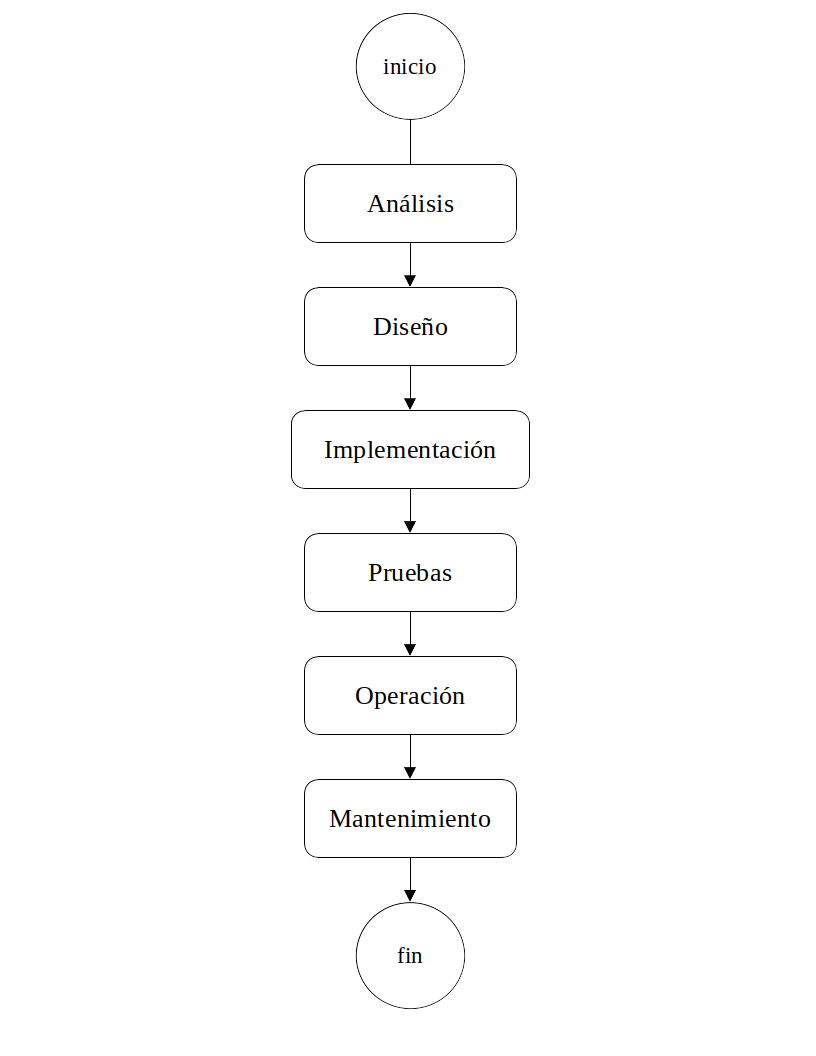
\includegraphics[height=20cm, clip]{/home/saikkopat/Documents/school/BD/TA2/diag.png}%
				}

\newpage

\textbf{Bibliografía}

\begin{enumerate}
	\item Database Lifecycle. (s/f) MariaDB KnowledgeBase. Recuperado el 22 de febrero de 2023, de \emph{https://mariadb.com/kb/en/database-lifecycle}.
\end{enumerate}

\end{document}